\section{Fundamentals of the Framework}
\label{sec:framework}

The framework proposed in this paper describes how and why to use \workshops. We use the term {\it framework} because what we have created provides an interpretive understanding and approach to practice instead of causal or predictive knowledge~\cite{Jabareen2008}. 
The framework is a thinking tool to navigate the process of planning, running, and analyzing a workshop, but we note that it cannot resolve every question about workshops because the answers will vary with local experience, preference, and context. In this section, we describe a set of factors that contribute to workshop effectiveness, as well as introduce the workshop process model and structure. 
We intend for the framework to be complemented by existing workshop resources from outside of visualization~\cite{CreativeEducationFoundation2015,Brooks-Harris1999,Gray2010,Hamilton2016}.

\subsection{Tactics for Effective Workshops}

Reflecting on our experience and reviewing the relevant literature~\cite{Nickerson1999,Osborn1953,Sawyer2003,Sawyer2006,Shneiderman2005} enabled us to identify several key factors that contribute to the effectiveness of workshops: focusing on the \topic of visualization, data and analysis, while fostering, maintaining, and potentially varying the levels of \agency, \collegiality, \trust, \interest, and \challenge associated with each. We term these factors {\bf \tactics for effective workshops}:  
\begin{itemize}[noitemsep,nolistsep]
\item \Tactic{T}{opic} --- the space of ideas relevant to data, visualization, and domain challenges in the context of the workshop theme.
\item \Tactic{A}{gency} --- the sense of stakeholder ownership in the workshop, the workshop outcomes, and the research collaboration.
\item \Tactic{C}{ollegiality} --- the degree to which communication and collaboration occur among stakeholders.
\item \Tactic{T}{rust} -- the confidence that stakeholders have in each other, the workshop, the design process, and the researchers' expertise.
\item \Tactic{I}{nterest} --- the amount of attention, energy, and engagement to workshop methods by the stakeholders.
\item \Tactic{C}{hallenge} --- the stakeholders' barrier of entry to, and likelihood of success in, workshop methods.
\end{itemize}

The \tactics are not independent, consistent, or measurable. The extent to which they are fostered depends upon the context in which they are used, including various characteristics of the workshop --- often unknown in advance, although perhaps detectable by facilitators. Yet, selecting methods to maintain appropriate levels of \agency, \interest, and \trust ~--- while varying levels of \challenge and approaching the \topic from different perspectives --- likely helps workshops to have a positive influence on the \mindset of stakeholders and to generate ideas that move forward the \methodology of the project. Hence, we refer to the \tactics throughout this framework.

\subsection{Process Model and Structure}
\label{sec:process-and-structure}

\begin{figure}
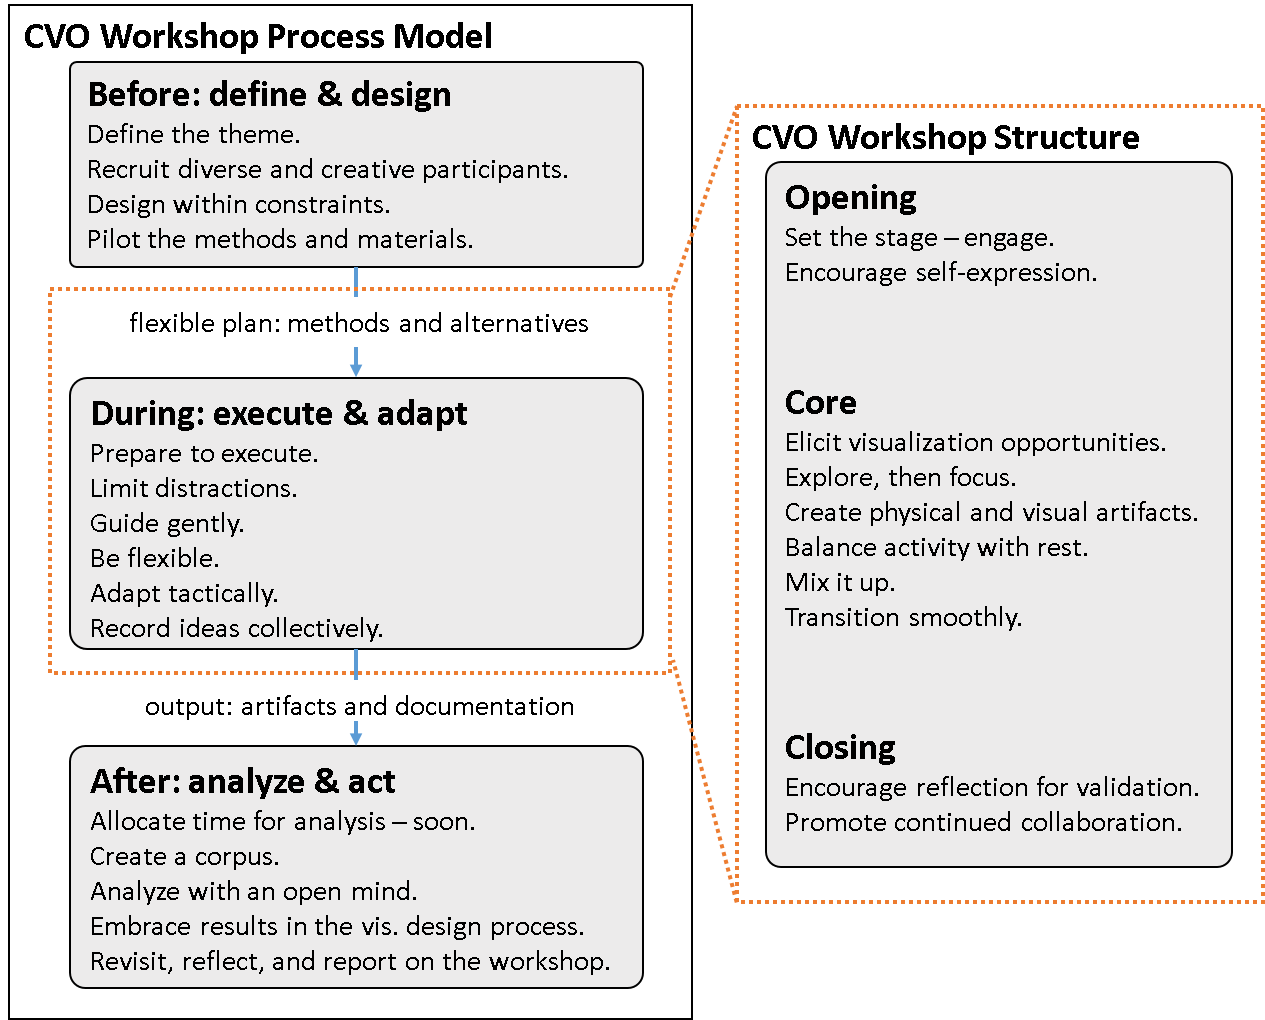
\includegraphics[width=\columnwidth]{figures/final.png}
\caption{The framework's two models are 1) a process model (left) that describes the common actions before, during, and after workshops; and 2) a structure that describes principles for methods used in the beginning, in the middle, and at the end of workshops. In these models, we propose \numberOfGuidelines guidelines for future workshops, summarized here.}
\label{fig:framework-overview}
\end{figure}

The framework proposes two models for describing how to use \workshops: a process model and a workshop structure. The models were adapted from the extensive literature that describes how to use workshops outside of visualization~\cite{CreativeEducationFoundation2015,Brooks-Harris1999,DeBono1983,Dove2016,Gray2010,Hamilton2016,Osborn1953}. 

The process model shown in Fig.~\ref{fig:framework-overview} (left) consists of three stages that describe the actions of using \workshops:
\begin{enumerate}[noitemsep,nolistsep]
    \item {\bf Before: define \& design.} Define the workshop theme and design workshop methods, creating a flexible workshop plan.
    \item {\bf During: execute \& adapt.} Perform the workshop plan, adapting it to participants' reactions in light of the \tactics, generating workshop output as a set of artifacts and documentation.
    \item {\bf After: analyze \& act.} Make sense of the workshop output and use it in the downstream design process.
\end{enumerate}

Nested within the process is the \workshop structure --- Fig.~\ref{fig:framework-overview} (right) --- that identifies key aspects of the methods used in the beginning, middle, and end of workshops:
\begin{enumerate}[nolistsep,noitemsep]
    \item {\bf Opening.} Establish shared context and \interest while promoting \trust, \agency, and \collegiality.
    \item {\bf Core.} Promote creative thinking about the \topic, potentially varying \challenge to maintain \interest.
    \item {\bf Closing.} Provide time for reflection on the \topic and promote continued \collegiality in the collaboration.
\end{enumerate}

The process model and structure are closely connected as shown by the orange box in Fig.~\ref{fig:framework-overview}. As part of the workshop process, we design and execute a workshop plan. This plan follows the workshop structure because it organizes methods into the opening, core, and closing. In other words, the process is about how we use a workshop; the structure is about how methods are organized within a workshop. 

We use the process model and structure to organize the following four sections of this paper. In these sections, we use paragraph-level headings to summarize \numberOfGuidelines actionable workshop guidelines. Additionally, in Supplemental Materials we include a complementary set of \numberOfPitfalls pitfalls that are positioned against these guidelines and the \tactics to further enhance the actionability of the framework.
